\section{Einführung}

\subsection{Prinzip der FM-Synthese}
Die Frequenzmodulationssynthese ist eine für die Musikwelt sehr wichtige Anwendung der Frequenzmodulation, welche bereits aus der Nachrichtentechnik bekannt ist. Generell wird dabei die Frequenz eines Trägersignals durch ein weiteres Modulationssignal verändert, die Amplitude bleibt jedoch unangetastet. Bei der FM-Synthese kann sich in besonderen Fällen jedoch auch die Amplitude des Modulierten Signals von dem ursprünglichen Trägersignals unterscheiden. In der Nachrichtentechnik können durch die unterschiedlichen Frequenzen im modulierten Trägersignal Informationen übertragen werden. 

Die momentane Amplitude des modulierten Signals lässt sich durch folgende Formel beschreiben:

\[
e(t) = A\sin(\alpha t + I\sin(\beta t)) \cite{chowningPaper}
\]

Bei der äußeren Sinusfunktion handelt es sich um das Trägersignal, welches in seiner Frequenz durch das Modulationssignal (Innerer Sinus) moduliert wird.

Abbildung \ref{fig:vergleichSignale} veranschaulicht die Frequenzmodulation eines Signals durch ein zweites Signal.

\begin{figure} [ht]
\centering
  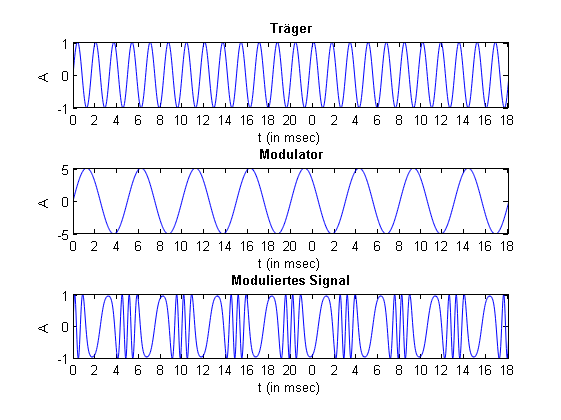
\includegraphics[width=0.95\textwidth,frame]{Prinzip.png}
\caption{Vergleich Träger/Modulator}
\label{fig:vergleichSignale}
Quelle: Eigene Darstellung mit Matlab
\end{figure}

Die Frequenzmodulationssynthese ist in ihren Grundzügen recht einfach zu verstehen und man kann mit geringem Aufwand bereits sehr komplexe, wenn auch oft unkontrollierbare Signale mit komplexen Klangspektren (bzw. Frequenzspektren) erzeugen. Wie sich im Folgenden jedoch noch herausstellen wird, ist es dagegen sehr schwierig und erfordert viel Zeit und Aufwand, durch die FM-Synthese gezielt Signale zu erzeugen und diese zu kontrollieren.

Praktisch gesehen kann die Frequenzmodulationssynthese dazu verwendet werden, um zum Einen Klangbilder echter Instrumente digital nachzubilden, jedoch auch um ganz neue Töne zu erzeugen, die so in der realen Welt nicht vorkommen.

\subsection{Beispiele}
In diesem Kapitel werden einige konkrete Beispiele der FM-Synthese anhand von Träger- und Modulationsfunktion sowie der daraus resultierenden Funktion aufgezeigt. Die Grafiken zeigen jeweils Plots von allen drei Signalen, welche mit Matlab erzeugt wurden.
Die Frequenzen der jeweiligen Funktionen wurden so gewählt, dass sie in einem Frequenzbereich liegen der vom menschlichen Ohr wargenommen werden kann. (Siehe Unterkapitel ``\ref{}'' im Kapitel ``\ref{}).

\begin{figure} [ht]
\centering
  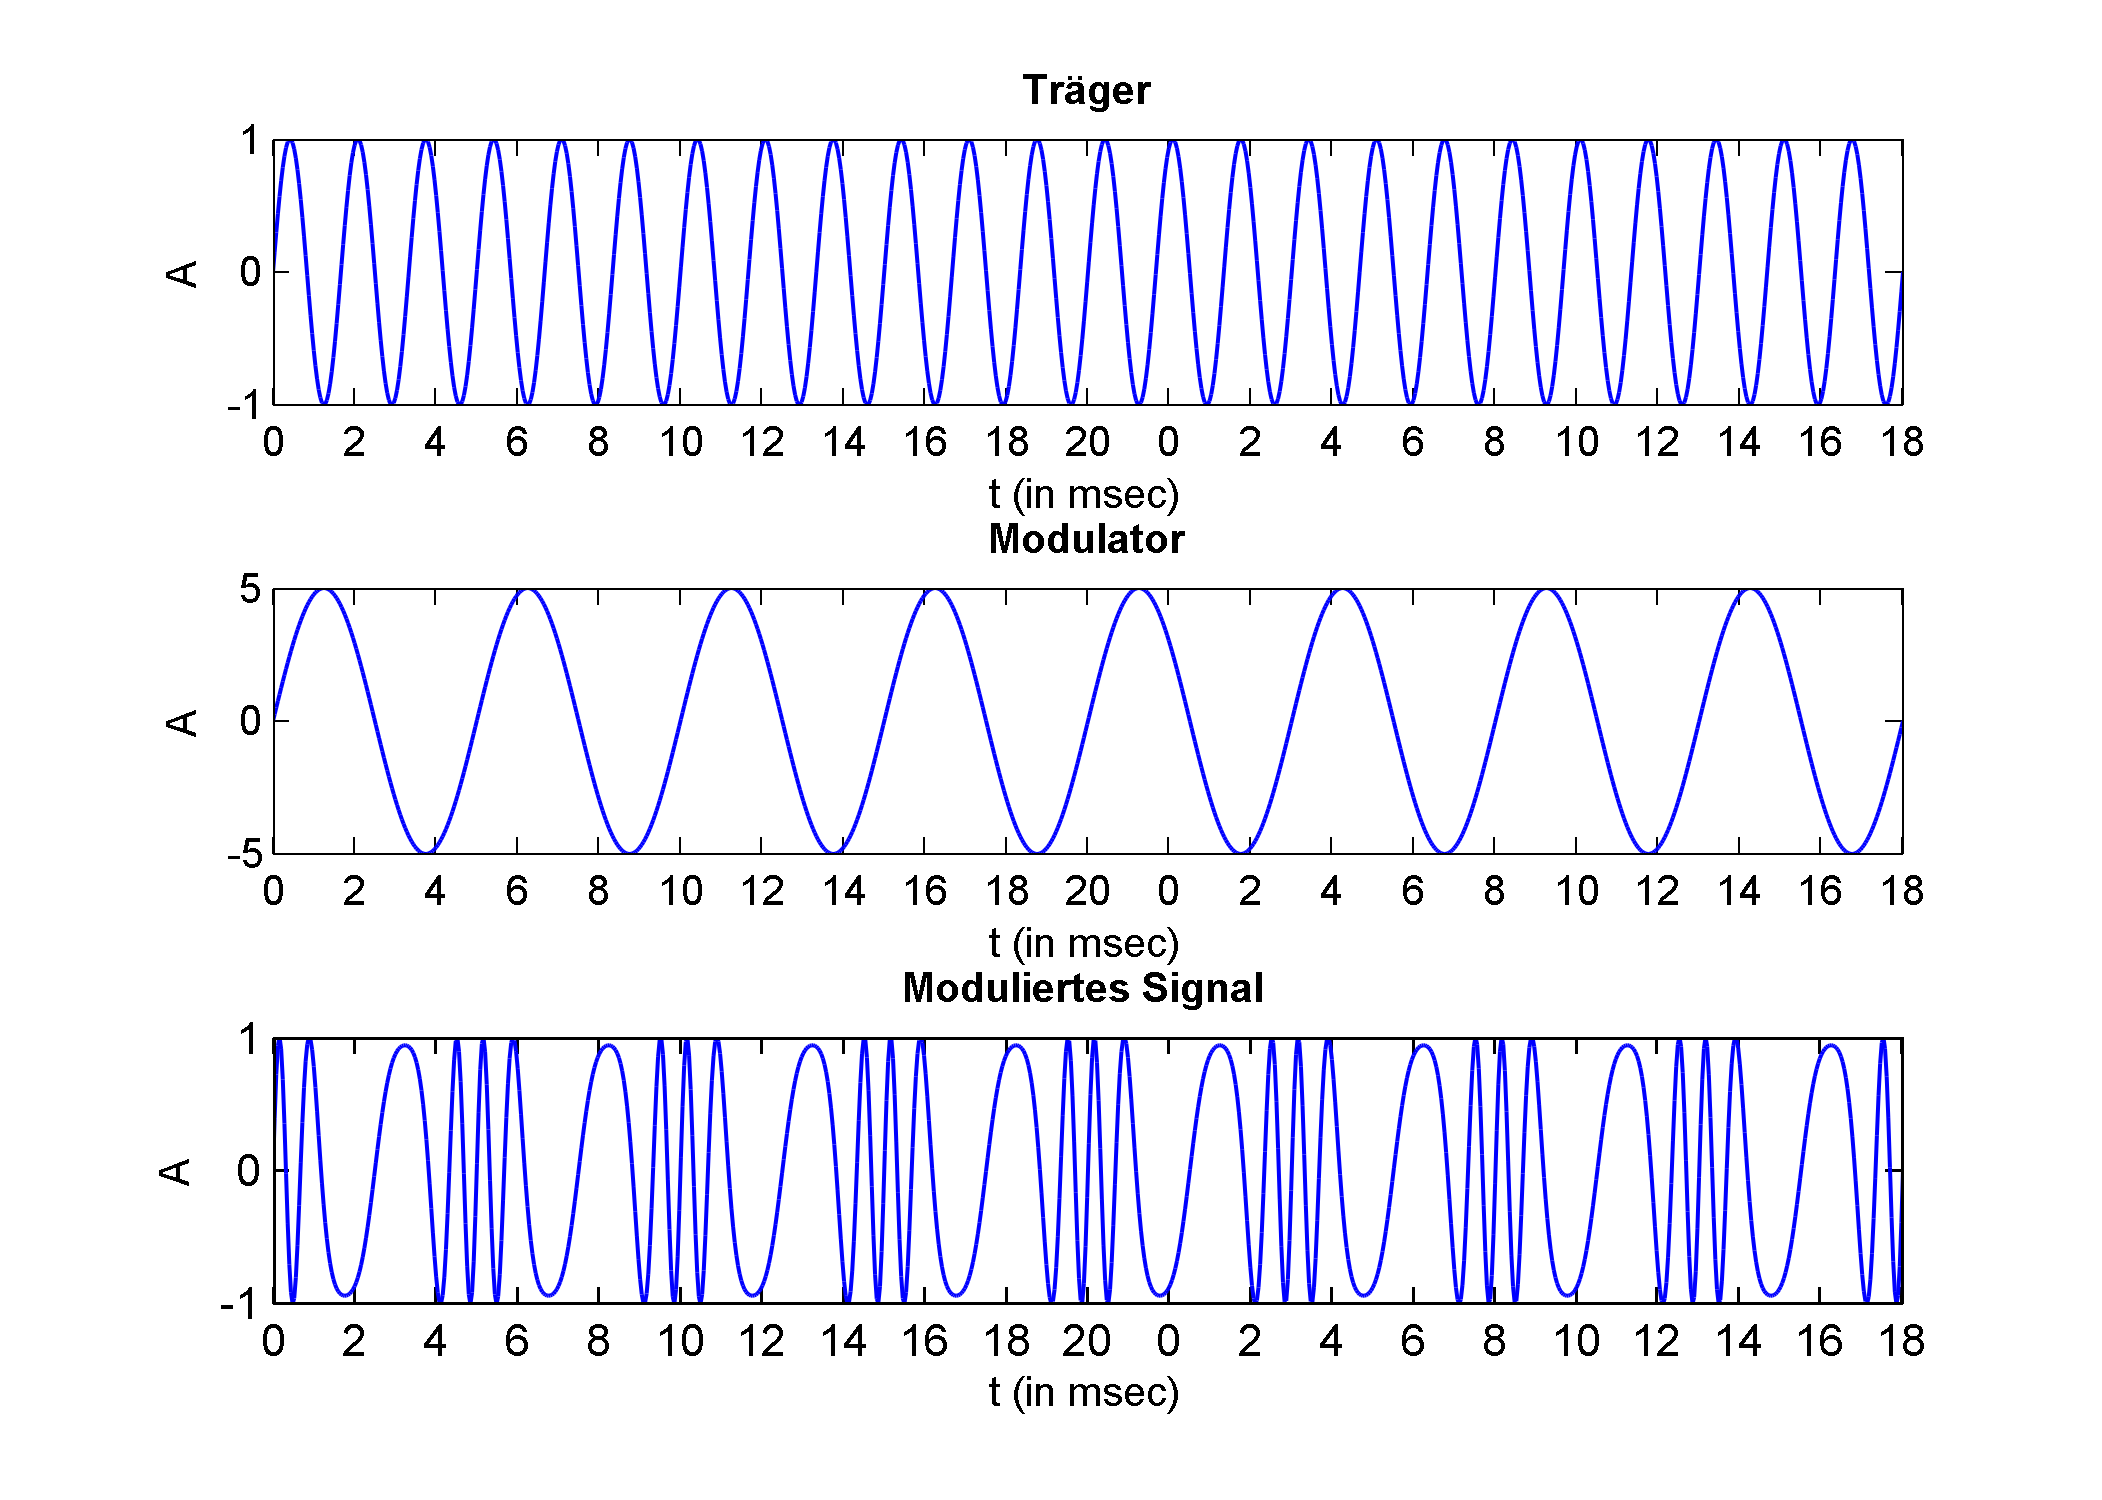
\includegraphics[width=0.95\textwidth,frame]{Beispiel1.png}
\caption{Beispiel 1}
\label{fig:beispiel1}
Quelle: Eigene Darstellung mit Matlab
\end{figure}

In Beispiel 1 (siehe Abbildung \ref{fig:beispiel1})  wurden folgende Signale verwendet:

\begin{lstlisting}[mathescape]
Trägersignal: 		$y(t) = \,\;\;\sin(2 \pi 600*t)$
Modulator:		$y(t) =5 \sin(2 \pi 75*t)$
Gesamtfunktion: 	$y(t) = \,\;\;\sin(2 \pi 600*t + 5 \sin(2 \pi 75*t))$
\end{lstlisting}

Konkrete Bedeutung der Werte: Die Trägerfrequenz von 600 Hz bedeutet, dass die Trägerfunktion 600 mal pro Sekunde schwingt, d.h. eine Periode ist genau $\frac{1}{600}$ Sekunden lang. Der Modulator hat eine Frequenz von 75 Hz, wodurch er 75 Schwingung pro Sekunde macht und eine Periode dann $\frac{1}{75}$ Sekunden lang ist. Für die Modulation gilt im Allgemeinen, dass der sogenannte Frequenzhub der Modulation (Erklärung siehe Kapitel ``\nameref{technisches}'') immer dann Maximal ist (in positiver oder negativer Richtung), wenn die Änderung der Modulationsfunktion (also deren Steigung) ihr Maximum bzw. Minimum hat. In der Grafik ist das immer dann der Fall, wenn der Modulator den Funktionswert 0 hat.

\begin{figure} [ht]
\centering
  \includegraphics[width=0.95\textwidth,frame]{Beispiel2.png}
\caption{Beispiel 2}
\label{fig:beispiel2}
Quelle: Eigene Darstellung mit Matlab
\end{figure}

Das zweite Beispiel in Abbildung \ref{fig:beispiel2} zeigt eine Frequenzmodulation, bei der sich auch die Amplitude des Signals ändert. Dies geschieht rein durch die Phasenverschiebung des äußeren Sinus durch den Modulator, die tatsächliche Amplitude der Funktion bleibt dabei unangetastet. Der Träger hat in diesem Beispiel eine Frequenz von 300 Hz, der Modulator 120 Hz. Der Modulationsindex beträgt wieder 5. Die Formel des Modulierten Signals sieht wie folgt aus:

\[
y(t) = \sin(2 \pi 300*t + 5 \sin(2 \pi 120*t))
\]

An diesem Beispiel kann man sehr gut erkennen, dass die FM-Synthese mit wenig Aufwandt komplexe Signale erzeugen kann, diese jedoch schlecht kontrollierbar bzw. erklärbar sind.

Als gute akustische Beispiele für die Anwendung der FM-Synthese in der Musikwelt können die Stücke ``Sabelith'' und ``Turenas'' von John Chowning selbst genannt werden. Beide Stücke wurden ausschließlich mit FM-Synthese erzeugt und beinhalten viele verschiedene Klangarten sowie Instrumente.

\subsection{Geschichte der FM-Synthese}
Die Grundlegende Technik hinter der FM-Synthese stammt, wie bereits erwähnt, aus der Nachrichtentechnik. Dort wird das Verfahren ``Frequenzmodulation'' genannt. Prof. Dr. John Chowning selbst gibt als Quelle zu seiner Entdeckung das Buch ``Radio Engineering'' von Frederick Emmons Terman aus dem Jahre 1947 an \cite[s. xy]{soundofinnovation}. Im Jahr 1967 entdeckte John Chowning eine neue Eigenschaft der Frequenzmodulation. Während er mit unterschiedlichen Modulationsfrequenzen experimentierte und dabei verschiedene Vibrato erzeugte (unter Vibrato versteht man einen schwingenden Ton, d.h. eine pulsierende Änderung des Tons), verschwand der Vibrato plötzlich bei höheren Modulationsfrequenzen und Obertöne wurden hörbar, die sich vom eigentlichen Trägersignal abhebten.\cite{fatherofdigitalmusik}

Chowning selbst war sehr erstaunt über die entstandenen Töne. In einem Interview von 2005 sagte er dazu: 

``I was experimenting with just a sinusoid and kept increasing the vibrato rate, so all of a sudden it didn't sound like listening to a change in pitch in time, but rather i began to hear timbral differences. So the vibratio became very, very fast, hundreds of times per second, and very, very deep, as if the violinist had a different fingerboard, and the finger was whipping up and down at very high rates and very great distances. That would be sort of a physical metaphor for this.''\cite[s. xy]{soundofinnovation}

Es dauerte weitere 3 Jahre, bis Chowning die mathematischen Zusammenhänge hinter seiner Entdeckung vollständig ergründet hatte. Bis dahin war er außerdem bereits in der Lage, verschiedene Instrumente wie Trommeln oder Blasinstrumente nachzubilden. Da Chowning selbst leidenschaftlicher Komponist war, veröffentlichte er im Jahre 1971 sein erstes, rein durch FM-Synthese generiertes Stück mit dem namen ``Sabelithe''. Sein zweites Stück, ``Turenas',' folgte ein Jahr später.
Um die Stärken seiner neuen Technik zu demonstrieren, verwandelt Chowning beispielsweise in ``Sabelithe'' den Klang einer Trommel in den einer Trompete.\cite[s. xy]{soundofinnovation}
 
\begin{figure} [ht]
\centering
  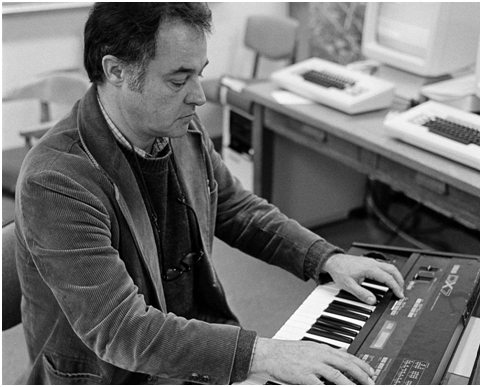
\includegraphics[width=0.95\textwidth]{chowning_CCRMA.png}
\caption{John Chowning am CCRMA}
Quelle: \url{http://arts.mit.edu/wp-content/uploads/2014/07/ChowningYamaha.jpg}
\end{figure}
 
Da Prof. Chowning seine Entdeckung nicht auf eigenes Risiko hin patentieren lassen wollte, lies er dies durch das OTL (Stanford Office of Technology Licensing) durchführen. Er selbst sagte dazu:

``I didn’t want to deal with lawyers — I wanted to do my music. I didn’t care about the money as much as I cared for my compositions. It was natural for me to say, `Please take it.' ''\cite{fatherofdigitalmusik}

 Seine neue Entdeckung war jedoch zu Beginn nicht sehr angesehen und auch viele der Firmen, welchen das neue Patent angeboten wurde, wussten nichts damit anzufangen und lehnten ab. Andy Moorer, ein Kollege Chownings in Stanford und später Mitgründer des CCRMA, sagte dazu: ``[...] It was really discouraging. John was so proud of having put this damn thing together and people didn't really get he idea of spatializing the sound.''\cite[s. xy]{soundofinnovation}

Offiziell veröffentlichte John Chowning seine neue Entdeckung der Frequenzmodulations-Synthese in einem Paper, welches 1973 im ``Journal of the Audio Engineering Society'' unter dem Titel ``The Synthesis of Complex Audio Spectra by Means of Frequenzy Modulation'' erschien.

Erst im Jahr 1974, als ein junger Ingeneur namens Kazukiyo Ishimura von der Firma Yamaha zu einer Vorstellung des Verfahren geschickt wurde, erkannte dieser binner wenigen Minuten, welches Potenzial hinter dieser neuen Anwendung der Frequentmodulation steckt. Yamaha Lizensierte das Verfahren noch im gleichen Jahr. Ishimura wurde später Chef des Yamaha Konzerns \cite{fatherofdigitalmusik}.

Im Jahr 1975, nach einiger Zeit Abwesenheit von Stanford, kehrte Chowning dorthin zurück und gründete zusammen mit einigen seiner Kollegen das CCRMA (Center for Computer Research in Music and Acoustics), welches sich auf Computermusik spezialisiert hat.
Eine Fotografie der Gründer von CCRMA ist auf Abbildung \ref{fig:foundersCCRMA} zu sehen.

\begin{figure} [ht]
\centering
  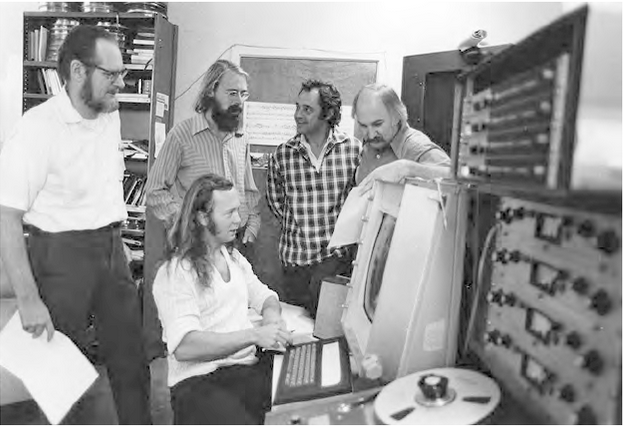
\includegraphics[width=0.95\textwidth]{Founders_CCRMA.png}
\caption{Gründer von CCRMA. Stehend von Links nach rechts: Leland Smith, John Grea, John Chowning und Loren Rush. Sitzend: Andy Moorer.}
\label{fig:foundersCCRMA}
Quelle: \cite{soundofinnovation} - Abbildung 4.1
\end{figure}

Nachdem Yamaha die Technik der FM-Synthese lizenziert hatte, brachten die Firma nach einem Prototypen im Jahre 1980 den ersten digitalen FM-Synthesizer GS1 und zwei Jahre später mit dem GS2 eine kleinere und handlichere Version des GS1 heraus. Die Geräte kosteten um die 30.000 DM für den GS1 bzw. 16.000 DM für den GS2 und waren deshalb nur für ausgewählte Musiker gedacht. Der Durchbruch gelang im Jahre 1983 mit dem DX7. Dieser konnte parallel 16 Stimmen verarbeiten und kostete ca. 4.700 DM. Preislich ähnliche und damals übliche analoge subtraktive Synthesizer konnten lediglich 4 Stimmen verarbeiten \cite{fmGS1}. Ein Bild des DX7 ist in Abbildung \ref{fig:dx7} zu sehen.

 \begin{figure} [ht]
\centering
  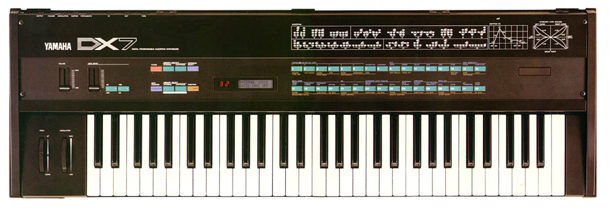
\includegraphics[width=0.95\textwidth]{dx7.png}
\caption{Yamaha DX7}
\label{fig:dx7}
Quelle: \url{http://www.electricdruid.net/images/interface/larger/YamahaDX7.jpg}
\end{figure}

Durch den großen Erfolg des DX7 konnte Yamaha in den nachfolgenden Jahren viele Weiterentwicklungen auf den Markt bringen. In den Jahren 1983 bis 1989 brachte Yamaha über 20 weitere digitale Synthesizer heraus. Über die Zeit wurden jedoch andere Syntheseverfahren günstiger und für den Markt besser geeignet, weshalb Yamaha 1990 mit dem SY77 Synthesizer ein Gerät entwickelte, das FM-Synthese und ein anderes digitales Klangsyntheseverfahren namens Sampling in einem vereinte.\cite{fmGS1}

Ab Mitte der 1990er wurden Personal Computer leistungsfähig genug, um Synthesizer ohne Verzögerung durch eine Midi Tastatur ansprechbar zu machen. Heutzutage findet digitale Audioverarbeitung nahezu ausschließlich softwareseitig statt, weshalb Hardwaresynthesizer wie der DX7 an Bedeutung verloren haben. Speziell dieser wurde jedoch durch die Firma Native Instruments in Form des FM7 und dessen Weiterentwicklung, dem FM8, in Software nachgebaut und findet heute noch Verwendung. Auch ist der DX7 heute bei Nostalgikern noch sehr beliebt.\cite{fmGS1}